\begin{figure}[h] 
\centering 
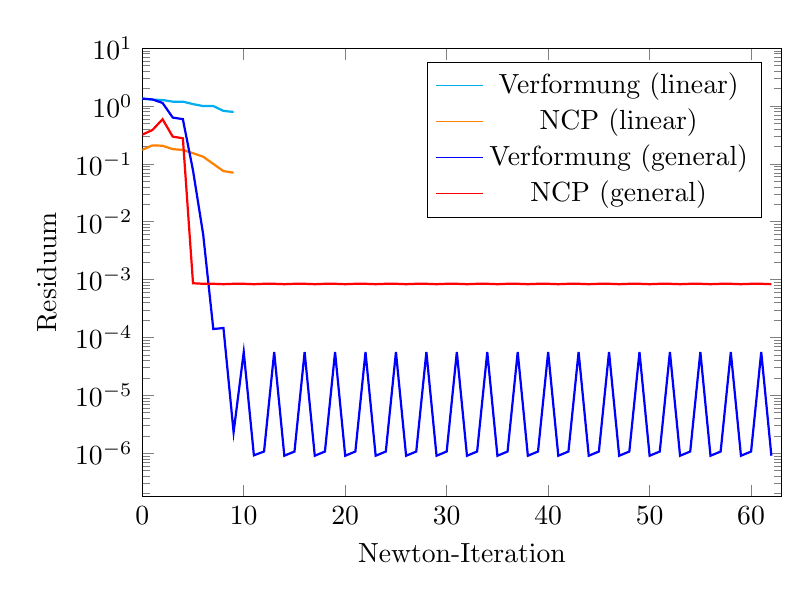
\begin{tikzpicture}[every plot/.append style={thick}] 
\begin{axis}[ 
label style={font=\normalsize}, 
xlabel={Newton-Iteration}, 
ylabel={Residuum}, 
xmin=0, xmax=63, 
ymode=log, 
ymin=0, ymax=10, 
width=0.8\textwidth, 
height=0.6\textwidth, 
legend pos=north east, 
legend style={cells={align=left}}, 
grid style=dashed, 
] 
\addplot[ 
color=cyan, 
] 
coordinates { 
(0, 1.35e+00)(1, 1.29e+00)(2, 1.27e+00)(3, 1.19e+00)(4, 1.19e+00)(5, 1.08e+00)(6, 9.98e-01)(7, 9.99e-01)(8, 8.24e-01)(9, 7.90e-01)}; 
\addlegendentry{Verformung (linear)} 
\addplot[ 
color=orange, 
] 
coordinates { 
(0, 1.75e-01)(1, 2.09e-01)(2, 2.06e-01)(3, 1.80e-01)(4, 1.74e-01)(5, 1.53e-01)(6, 1.33e-01)(7, 1.00e-01)(8, 7.51e-02)(9, 7.04e-02)}; 
\addlegendentry{NCP (linear)} 
\addplot[ 
color=blue, 
] 
coordinates { 
(0, 1.34e+00)(1, 1.30e+00)(2, 1.13e+00)(3, 6.32e-01)(4, 5.93e-01)(5, 7.70e-02)(6, 6.07e-03)(7, 1.40e-04)(8, 1.46e-04)(9, 2.31e-06)(10, 5.60e-05)(11, 9.20e-07)(12, 1.07e-06)(13, 5.60e-05)(14, 9.05e-07)(15, 1.07e-06)(16, 5.60e-05)(17, 9.05e-07)(18, 1.07e-06)(19, 5.60e-05)(20, 9.05e-07)(21, 1.07e-06)(22, 5.60e-05)(23, 9.05e-07)(24, 1.07e-06)(25, 5.60e-05)(26, 9.05e-07)(27, 1.07e-06)(28, 5.60e-05)(29, 9.05e-07)(30, 1.07e-06)(31, 5.60e-05)(32, 9.05e-07)(33, 1.07e-06)(34, 5.60e-05)(35, 9.05e-07)(36, 1.07e-06)(37, 5.60e-05)(38, 9.05e-07)(39, 1.07e-06)(40, 5.60e-05)(41, 9.05e-07)(42, 1.07e-06)(43, 5.60e-05)(44, 9.05e-07)(45, 1.07e-06)(46, 5.60e-05)(47, 9.05e-07)(48, 1.07e-06)(49, 5.60e-05)(50, 9.05e-07)(51, 1.07e-06)(52, 5.60e-05)(53, 9.05e-07)(54, 1.07e-06)(55, 5.60e-05)(56, 9.05e-07)(57, 1.07e-06)(58, 5.60e-05)(59, 9.05e-07)(60, 1.07e-06)(61, 5.60e-05)(62, 9.05e-07)}; 
\addlegendentry{Verformung (general)} 
\addplot[ 
color=red, 
] 
coordinates { 
(0, 3.20e-01)(1, 3.85e-01)(2, 5.91e-01)(3, 2.96e-01)(4, 2.77e-01)(5, 8.66e-04)(6, 8.47e-04)(7, 8.47e-04)(8, 8.34e-04)(9, 8.47e-04)(10, 8.47e-04)(11, 8.34e-04)(12, 8.47e-04)(13, 8.47e-04)(14, 8.34e-04)(15, 8.47e-04)(16, 8.47e-04)(17, 8.34e-04)(18, 8.47e-04)(19, 8.47e-04)(20, 8.34e-04)(21, 8.47e-04)(22, 8.47e-04)(23, 8.34e-04)(24, 8.47e-04)(25, 8.47e-04)(26, 8.34e-04)(27, 8.47e-04)(28, 8.47e-04)(29, 8.34e-04)(30, 8.47e-04)(31, 8.47e-04)(32, 8.34e-04)(33, 8.47e-04)(34, 8.47e-04)(35, 8.34e-04)(36, 8.47e-04)(37, 8.47e-04)(38, 8.34e-04)(39, 8.47e-04)(40, 8.47e-04)(41, 8.34e-04)(42, 8.47e-04)(43, 8.47e-04)(44, 8.34e-04)(45, 8.47e-04)(46, 8.47e-04)(47, 8.34e-04)(48, 8.47e-04)(49, 8.47e-04)(50, 8.34e-04)(51, 8.47e-04)(52, 8.47e-04)(53, 8.34e-04)(54, 8.47e-04)(55, 8.47e-04)(56, 8.34e-04)(57, 8.47e-04)(58, 8.47e-04)(59, 8.34e-04)(60, 8.47e-04)(61, 8.47e-04)(62, 8.34e-04)}; 
\addlegendentry{NCP (general)} 
\end{axis} 
\end{tikzpicture} 
\caption{Residuen des Stoffgesetzes 'St.Venant' mit Hinderniss 'Parabel' und 2178 Freiheitsgraden für die Verschiebung.} 
\label{fiq:St.Venant_Parabel_level4} 
\end{figure} 
